\documentclass{amsart} 
\usepackage{graphicx}
\graphicspath{{./}}
\usepackage[fontsize=14pt]{scrextend}
\usepackage{hyperref}
\usepackage{csvsimple}
\usepackage{epigraph}
\title{Fundamental Driver of Rapes is incapacity for Romantic Love}
\author{Zulfikar Moinuddin Ahmed}
\date{\today}
\begin{document}
\maketitle

I have in a previous note theorised that romantic love developed in human primate ancestors even before our evolution in bipedal primates with large brains.  When the infant primate brain is large enough the species cannot survive without paternal care which required romantic love and pair bonding.  

In this note I will offer some preliminary evidence that rapes are due primarily to incapacity in Romantic Love.  This is a subtle issue, for all human beings have evolutionary genomic capability for Romantic Love; however, various disruptions can lead to failures to develop the capacity for healthy Romantic Love relationships.

\section{Remarkable Low Rape Rates Globally}
The highest rape rates in the world are in Sweden, Iceland, United States, Belgium and Norway, and all other countries have lower rape rates.  But even in the highest case they occur for 0.06\% of the population.  In other words, 99.94\% of the men of Sweden do not commit any rapes for the entire year.  I have considered models to predict the rape rates elsewhere.  Here I focus on this remarkable universal regularity of rape rates.  We ought to find it quite astonishing that a natural species, the human race, ought to have men who are so well-behaved across the globe that rapes are committed uniformly by such an insignificant percent of men.  

Many hypotheses to explain rapes in the past did not stand on the universal regularity across the globe and therefore went astray into irrelevant variables.  We hypothesize that Romantic Love and its negation, various incapacities are responsible for the phenomena of rape.  These are much clearer in the large scale view.

\section{Stermac-Quinsey Social Competence Results}

Stermac-Quinsey \cite{SQ} have produced extremely clear discrimination of sexual offenders from other offenders and ordinary people in measures of social competence.

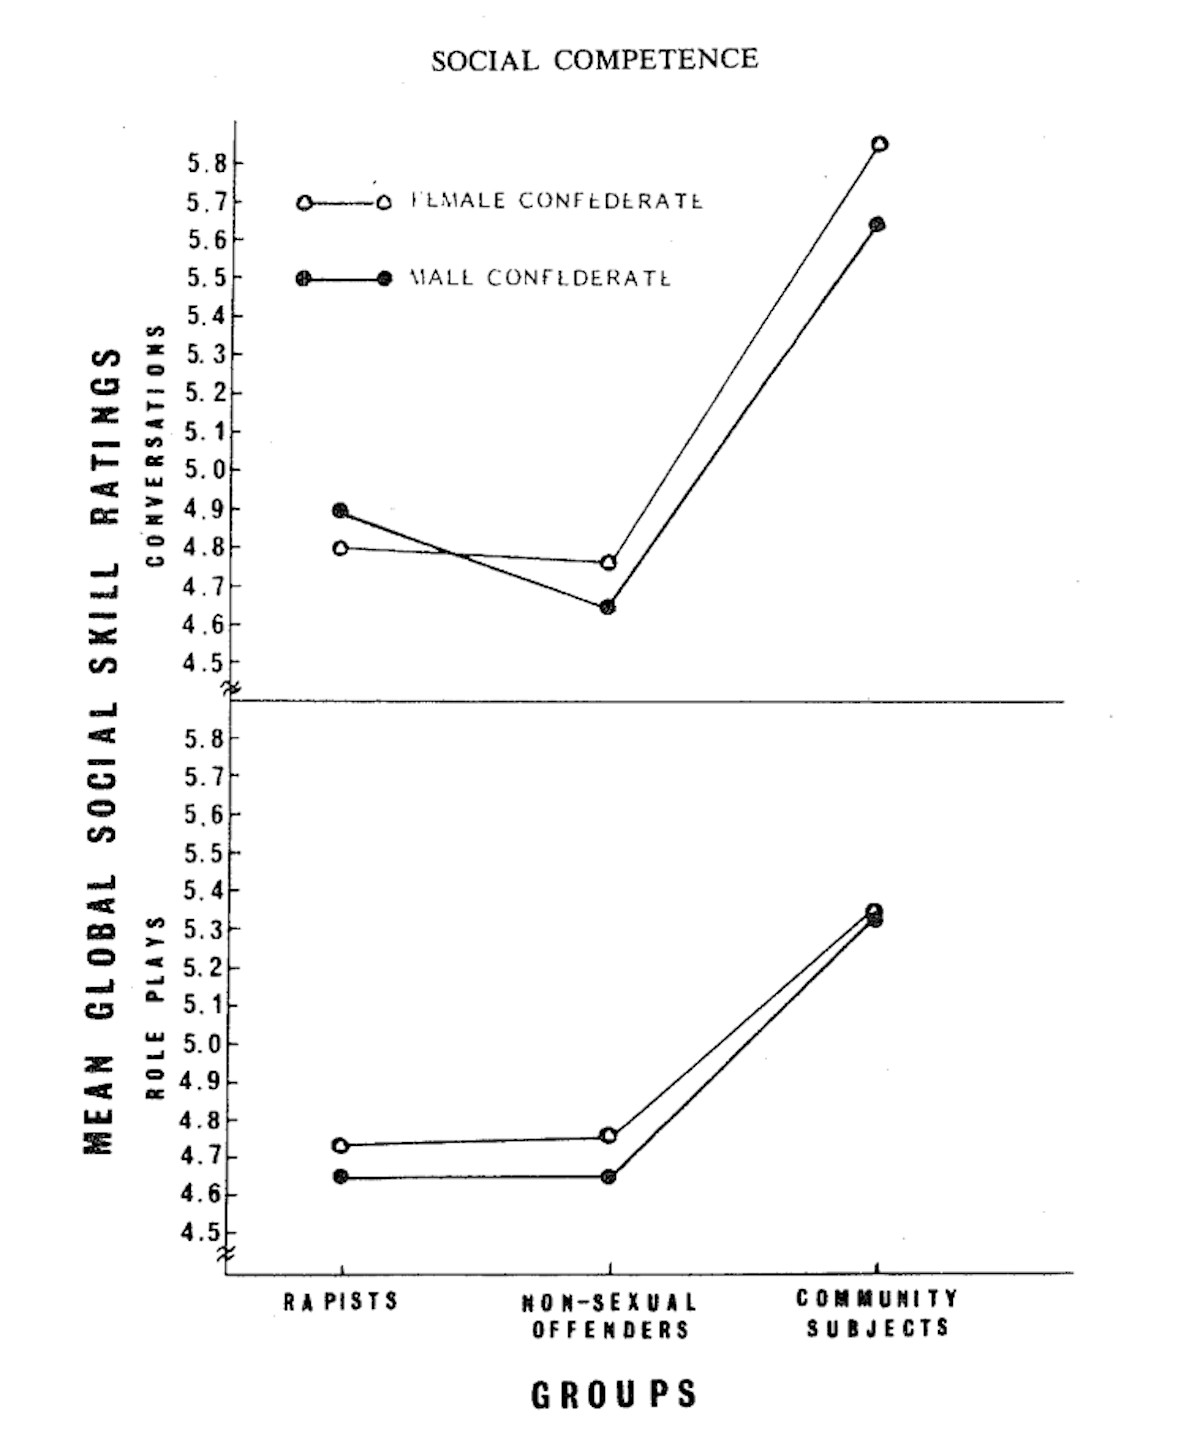
\includegraphics[scale=0.3]{rapistsocialcomp.jpeg}

\section{Low Childhood Attachment}

Mariana Reis \cite{Reis} measured the attachment security of sexual offenders.

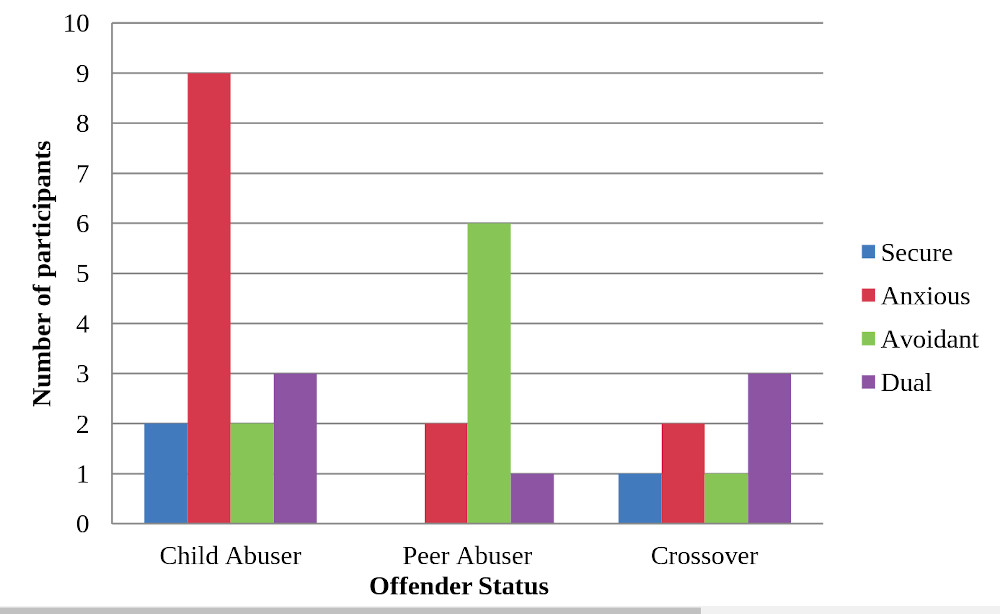
\includegraphics[scale=0.4]{rapistsec.jpeg}

\section{Proxies for Romantic Love Capacity}

Secure Attachment and Social Competence are, together, a rough proxy for capacity for Romantic Love.  There are numerous studies to support this.  The revolutionary claim made here is that the driving factor for Rapes around the world is only Romantic Love capacity and all other factors are nuisance parameters and less important.  In particular, we claim that various ethnic, national, and other factors are all secondary.  This is a very non-trivial claim, for we are able to produce nontrivial results for effect of log-GDP to explain rape rates.  Nevertheless, we still claim that the fundamental driver is still incompetence in Romantic love, and some of this might be absorved by a significant effect of log-GDP (per capita).



\begin{thebibliography}{CCC}
\bibitem{SQ}{L. Stermac and V. Quinsey, "Social Competence Among Rapists",{\em Behavioral Assessment, 1986}
\bibitem{Reis}{Mariana Reis, {\em Exploring the Attachment Style of Sex Offenders}, Ph.D. University of Birmingham, 2015.}
\end{thebibliography}
\end{document}
